% !Mode:: "TeX:UTF-8"

\documentclass{mcmthesis}
\mcmsetup{CTeX = false,   % 使用 CTeX 套装时,设置为 true
	tcn = {\color{red}67859}, problem = {\color{red}D}
	%        }
	,
	sheet = false, titleinsheet = true, keywordsinsheet = true,
	titlepage = true, abstract = true}
\usepackage{palatino}
\usepackage{enumitem} % Required for manipulating the whitespace between and within lists
\usepackage{listings}
\usepackage{multirow}
\usepackage{nicefrac}
\usepackage{sectsty}
\sectionfont{\color{MidnightBlue}\selectfont}
\subsectionfont{\color{MidnightBlue!50!RoyalBlue}\selectfont}
\subsubsectionfont{\color{SkyBlue!5!RoyalBlue}\selectfont}
\usepackage{booktabs}
\usepackage{lipsum}
\usepackage{varioref} % More descriptive referencing
\setlength\parindent{0pt}
\usepackage{subfig}
%\usepackage[UTF8,nocap]{ctex}
%\usepackage[subfigure,titles]{tocloft}
\usepackage[subfigure]{tocloft}
%\renewcommand\cftsecfont{\color{MidnightBlue}}
%\renewcommand\cftpartpagefont{\color{RoyalBlue}}
%\setlength\cftbeforesecskip{-4pt}
%\setlength\cftbeforesubsecskip{-3.3pt}
%\setlength\cftbeforesubsubsecskip{-5.2pt}
%\renewcommand\cftsecafterpnum{\vskip-4pt}
%\renewcommand{\cftsubsecafterpnum}{\vskip-3.3pt}
%\renewcommand{\cftsubsubsecafterpnum}{\vskip-5.2pt}
%\usepackage[round]{natbib}
%\bibliographystyle{plainnat}
\usepackage{mmstyles}
\usepackage{longtable}
\usepackage{pdflscape}
\usepackage{graphicx}


%\usepackage{subfig} % Required for creating figures with multiple parts (subfigures)
%\usepackage{subfigure}
%\usepackage[square,sort,comma,numbers]{natbib}


\title{Solve Symmetric TSP using ILP}
\author{{\itshape Xinglu Wang} \quad {\itshape 3140102282} \quad {\itshape ISEE 1403, ZJU}}
\begin{document}

\maketitle
 
\setcounter{tocdepth}{2} % Set the depth of the table of contents to show sections and subsections only
\tableofcontents
		
\section*{Abstract }
In this report, I first formulate Traveling Salesman Problem(TSP) as  Integer Linear Program(ILP), then collect data for landmarks around HangZhou, use SageMath to solve the ILP, get the exact solution. 

\textbf{Keywords:} TSP, ILP
\section{Formulation}
TSP is a combinatorial optimization problem to find the shortest possible hamiltonian circuit for a complete weighted graph. % \vref{tab:ok}
\subsection{Definition}	 
\begin{table} 
	\centering
	{\begin{tabular}{c|l} 
	\hline
	$\vs = (s_i)$ & At $i$ step, the index of visited city is $s_i$, $ 0 \le i \le n-1$\\
	$\vt= (t_i)$ & City $i$ is visited at step $t_i$, $ 0 \le i \le n-1$\\ \hline \hline
	$\mX = (x_{i j} )$ & Decision variable, $x_{ij}={\begin{cases}1&{\text{the path goes from city }}i{\text{ to city }}j\\0&{\text{otherwise}}\end{cases}}$  \\
	$\pi(\cdot )$ & $\pi(i)=j  \text{ if } x_{i j}=1$, $ 0 \le i,j \le n-1$ \\ \hline \hline
	$\mC=(c_{ij})$ & Cost Matrix \\ 
	\hline
	\end{tabular}
	\caption{The notation that will be used}
	\label{tab:ok}}
\end{table}

There are several key elements:
\begin{itemize}
	\item Hamiltonian circuit means starting from vertex No. 0, ending at No. 0 and travel all vertexes once and only once. Note that $x_{ij}|_{i=n-1,j=0}$ will consider go back while  $t_i$ will not consider the time consumed when go back since there is \textit{no} $t_i|_{i=n}$.
	\item For a real-world problem, the weights for graph are non-negative. But the weights do no necessarily be symmetric, because weights can be time or cost. I choose \textit{unsymmetrical}  TSP to solve for its generality. Thus, I should note that $\mC$ is symmetric because the data I collect is distance while the solution $\mX$ is unsymmetrical because it describe \textit{directed} graph.
\end{itemize} 

\subsection{ILP formulation}
We formulate this question step by step, first we list all sufficient constrains:

\begin{align}
\mathop{\mathrm{Minmize \ \  }}       & \sum _{i=0}^{n-1}\sum _{j=0,{\color{Red} j\neq i}}^{n-1}c_{ij}x_{ij} &  & \label{eq:obj}          \\
\mathop{\mathrm{subject \  to \ \  }} & \sum _{i=0,i\neq j}^{n-1}x_{ij}=1                          &  & j=0,\ldots ,n-1;   \label{eq:row}       \\
& \sum _{j=0,j\neq i}^{n-1}x_{ij}=1                          &  & i=0,\ldots ,n-1;         \label{eq:col} \\
& x_{ij} \geq 0, x_{ij} \in \Zbb                                           &  & i,j=0,\ldots ,n-1. \notag
\end{align}

The objective function \eqref{eq:obj} need to minimize costs, we simply drop $x_{ii}$ throughout the problem, since $x_{ii}=0$ is trivial. The constrains \eqref{eq:row} means each city be arrived at from exactly one other city while equation \eqref{eq:col} means from each city there is a departure to exactly one other city. We do not need to add $x_{ij} \le 1 $ since others are enough to conclude it. 

But these constraints are not necessary conditions for TSP. This formulation in fact the formulation of Assignment Problem belong to P hard class. We still need to add constraints to avoid subtour and we will find that TSP belong to NP hard level class. I choose to add $n$ auxiliary variables so that I just need to add $n(n-1)$ constrain. 
\begin{align}
	\mathop{\mathrm{Minmize \ \  }}       & \sum _{i=0}^{n-1}\sum _{j=0,j\neq i}^{n-1}c_{ij}x_{ij} &  & \notag                     \\
	\mathop{\mathrm{subject \  to \ \  }} & \sum _{i=0,i\neq j}^{n-1}x_{ij}=1                    &  & j=0,\ldots ,n-1;  \notag     \\
	                                      & \sum _{j=0,j\neq i}^{n-1}x_{ij}=1                    &  & i=0,\ldots ,n-1;      \notag \\
	                                      & \color{Blue} t_{j} \ge t_{i}+1-n(1-x_{ij})x  &  & 0\leq i\leq n-1, {\color{Red}1 \le} j \le n-1, i \neq j   \label{eq:new}     \\
	                                      & x_{ij} \geq 0, x_{ij} \in \Zbb                     &  & i,j=0,\ldots ,n-1. \notag
\end{align}
Note that $j \ge 1 $ in \eqref{eq:new} means we do not consider salesman going back to No.0. In fact, if we let $t_{n}$ denote the time step salesman go back to No.0, we have:
\begin{equation}\label{eq:my}
t_{n}=t_{n-1}+1=n 
\end{equation}
 To prove correctness.  First, Cyclic permutation without subtour conclude \eqref{eq:new}. Because \eqref{eq:new} is equivalent to statement that   if the next visited city for $i$ is $j$ ($x_{ij}=1$) ,then $t_j=t_i+1$. If $x_{ij}=0$, then we add a trivial constraint $t_j \ge t_j +1-n$.  The equivalent statement is satisfied. Second, \eqref{eq:new} eliminates all subtour. We can prove it by tricky contrapositive. Suppose the feasible solution $\mX$ contain more than one subtour. Then there exist $\vs=(i_1,\dots,i_r)$ not containing 0. Note that $i_r$ in this circle will go back to $i_1$, so there is additional equation $t_{i_1}=t_{i_r}+1$  quite different with \eqref{eq:my}. Go along this cycle, we find that $0=r$, and the contradiction lies in the fact that the cycle do not containing 0.

\section{Experiments}

The steps to solve the ILP include: prepare location data for landmarks around HangZhou, solve the ILP by MILP class and visualize the final results on Map. The equivalent code for \eqref{eq:new} is shown below:

\begin{lstlisting}[language=Python]
p=MixedIntegerLinearProgram(maximization=False) 
# Define Varibles:
x=p.new_variable(nonnegative=True,integer=True)
t=p.new_variable(nonnegative=True,integer=True)
n=dist.nrows()
obj_func=0
# Define Obj Function:
for i in range(n):
	for j in range(n):
		obj_func+=x[i,j]*dist[i,j] if i!=j else 0
p.set_objective(obj_func)
# Add Constrains
for i in range(n):
	p.add_constraint(sum([x[i,j] for j in range(n) if i!=j ])==1)
for j in range(n):
	p.add_constraint(sum([x[i,j] for i in range(n) if i!=j ])==1)
for i in range(n):
	for j in range(1,n):
		if i==j :
			continue
		p.add_constraint(t[j]>=t[i]+1-n*(1-x[i,j]))
for i in range(n):
	p.add_constraint(t[i]<=n-1)

#p.show()
p.solve()
\end{lstlisting}

Apply ILP to a toy case with 20 landmarks around HangZhou, we get a optimal strategy to travel around HangZhou, which is quite interesting. Ref. to Fig~\vref{fig:tsp_res}. Then I also use TSP solver in Sage to partially verify that my code is correct. The approximate optimal solution got by some heuristic algorithm is the same as the exact optimal solution. The I try to not just travelling Hangzhou, and travel JiangZheHu Region(Yangtze River delta). Visualized on the map, Ref. to Fig~\vref{fig:jiangzhehu}. 

\begin{figure}
	\centering
	\subfloat[Initial feasible solution for TSP]{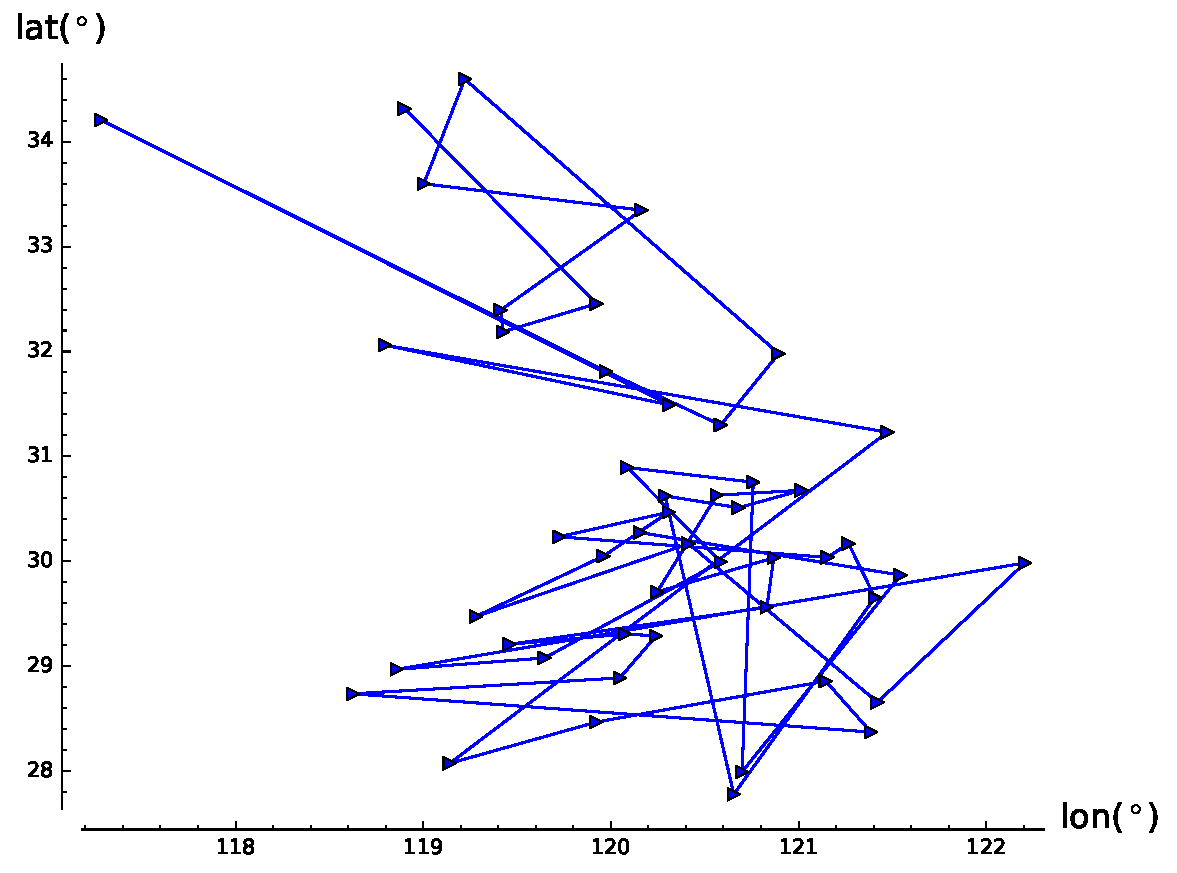
\includegraphics[width=.4\columnwidth]{init_map}} \quad  
	\subfloat[Transform into complete weight graph]{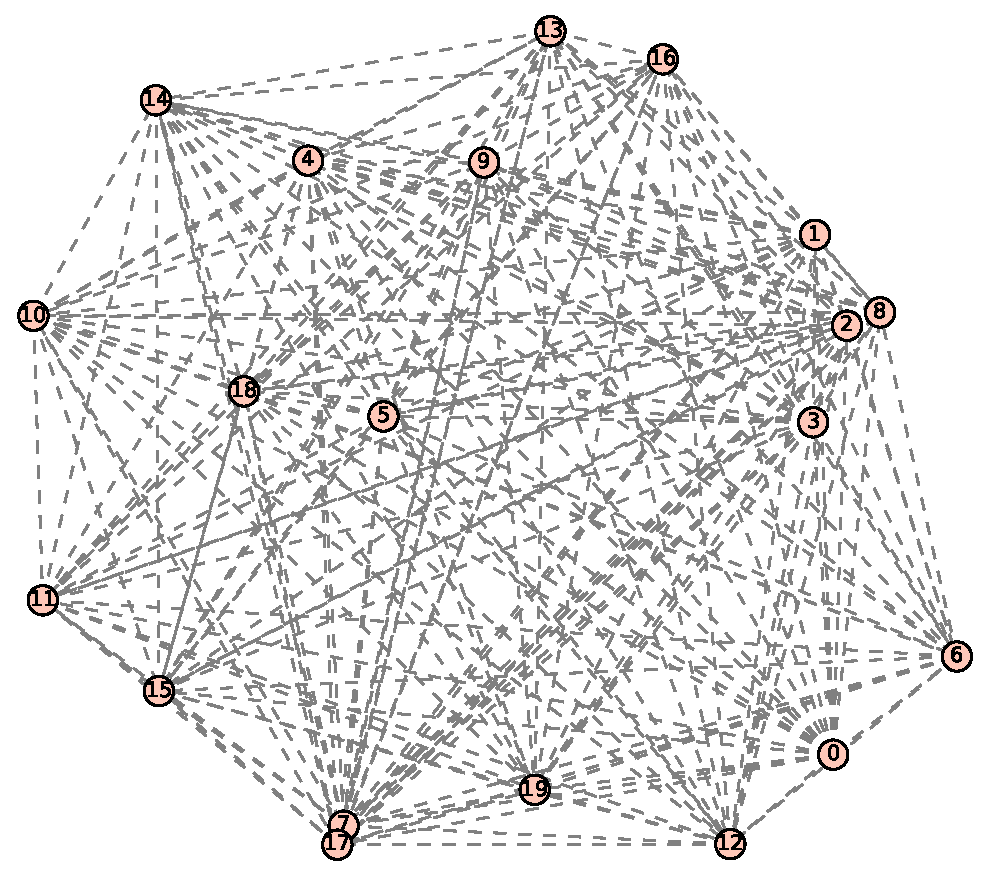
\includegraphics[width=.4\columnwidth]{topology}} 
	\\
	\subfloat[The optimal solution find by ILP]{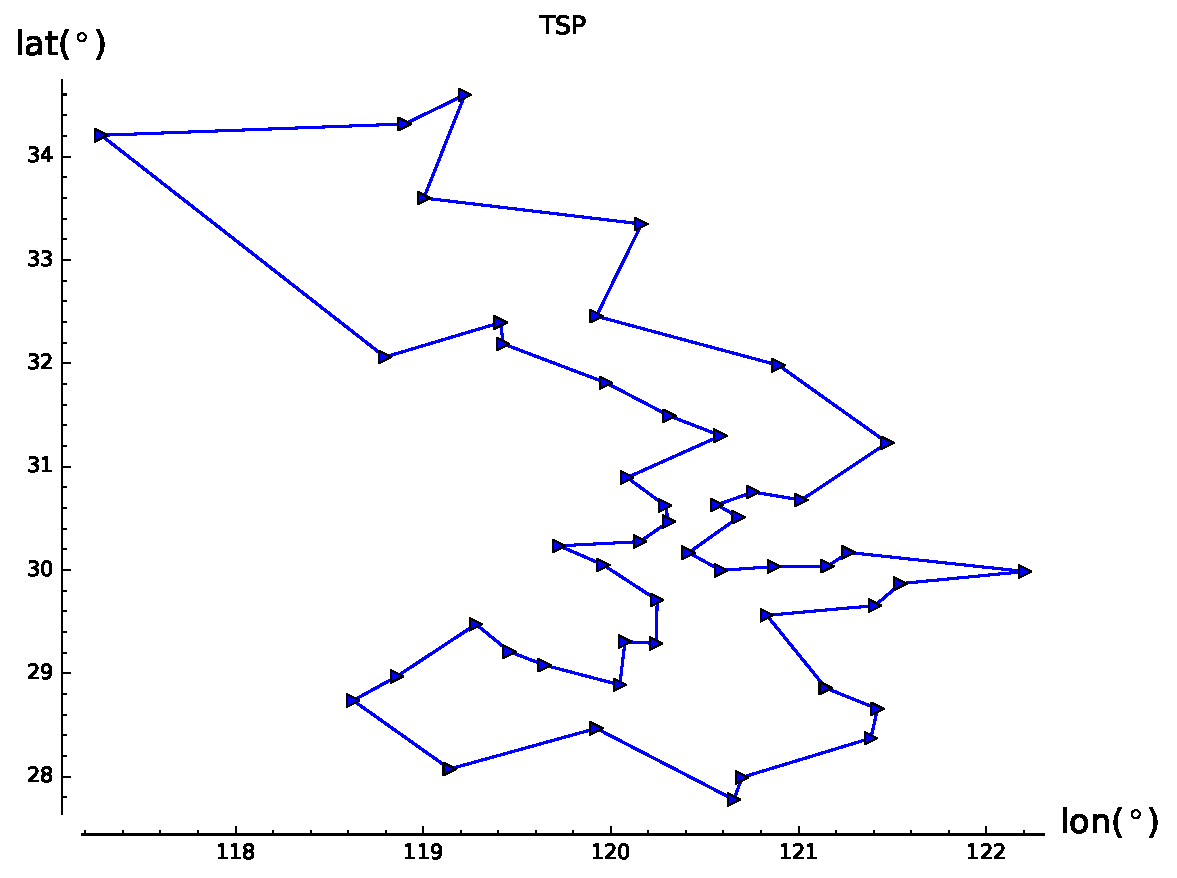
\includegraphics[width=.4\columnwidth]{tsp_res}\label{fig:tsp_res}}  \quad 
	\subfloat[Approximately optimal find by Sage]{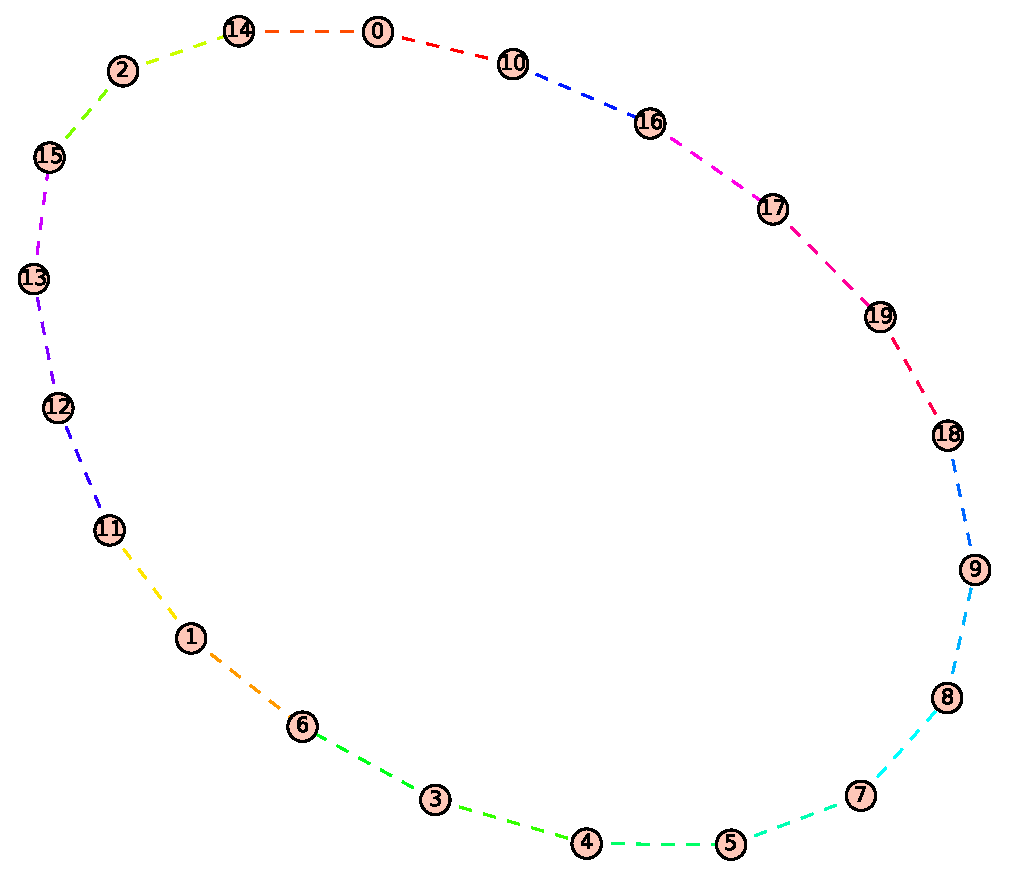
\includegraphics[width=.4\columnwidth]{tsp_sage} \label{fig:tsp_sage} }
	\caption[Results]{The plot  of  TSP class \vref{fig:tsp_sage} only keep topological relations, but after simple transformation, we find for 20-pts, two solutions $\mX$ are equivalent. (Here the transformation means change from undirected graph's $\mX=(x_{ij})$ with $i < j$  to directed graph's $\mX$ ) } 
\end{figure}
\begin{figure}
	\centering
	\subfloat[TSP on Hangzhou]{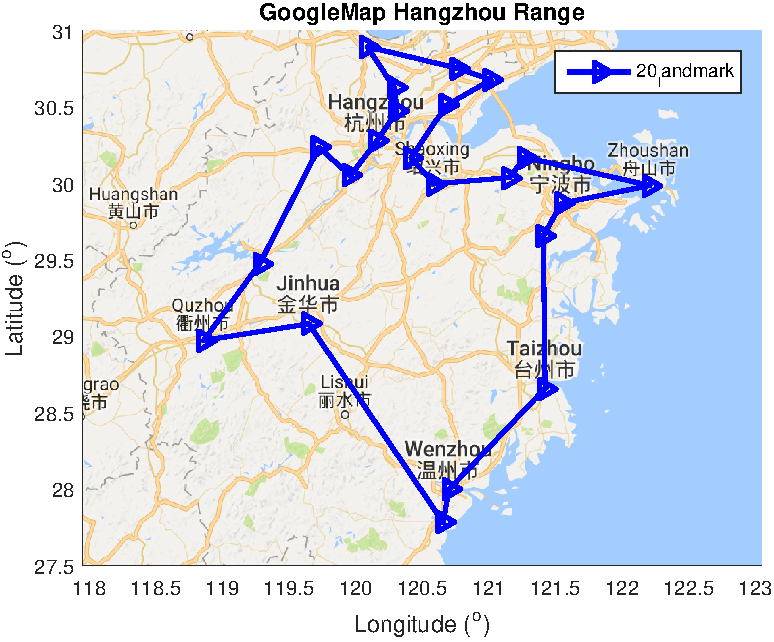
\includegraphics[width=.48\columnwidth]{GMap}} \   
	\subfloat[TSP on JiangZheHu]{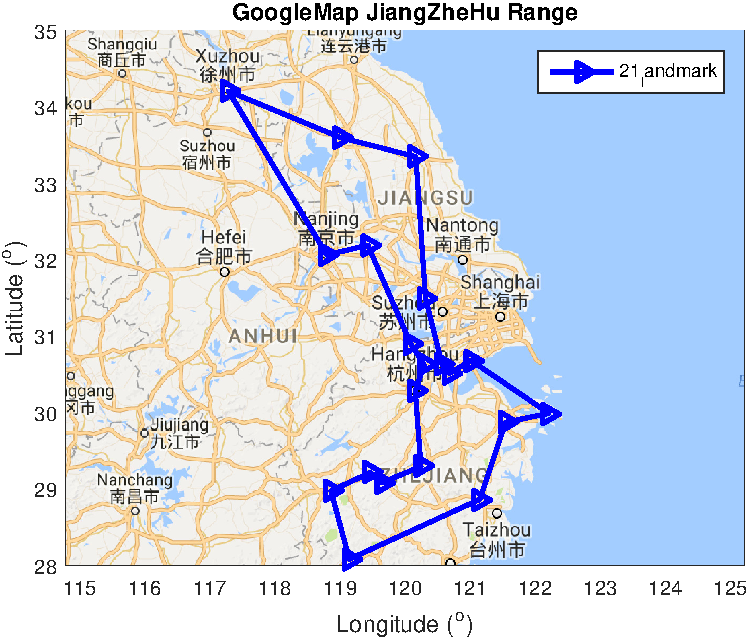
\includegraphics[width=.47\columnwidth]{GMap_Jzh}\label{fig:jiangzhehu}} 
	\caption[Results]{JiangZheHu is a wider range than Hangzhou. We limit number of landmarks to about 20 for speed.} 
\end{figure}

I just take 20 landmarks from 49 collected coordinate data. The reason lies in I find 50 points consume seemingly endless time. I also have some basic test on running time, and find it grow explosively. Ref. to Fig~\vref{fig:elaspe}

\begin{figure}[h]
	\centering
	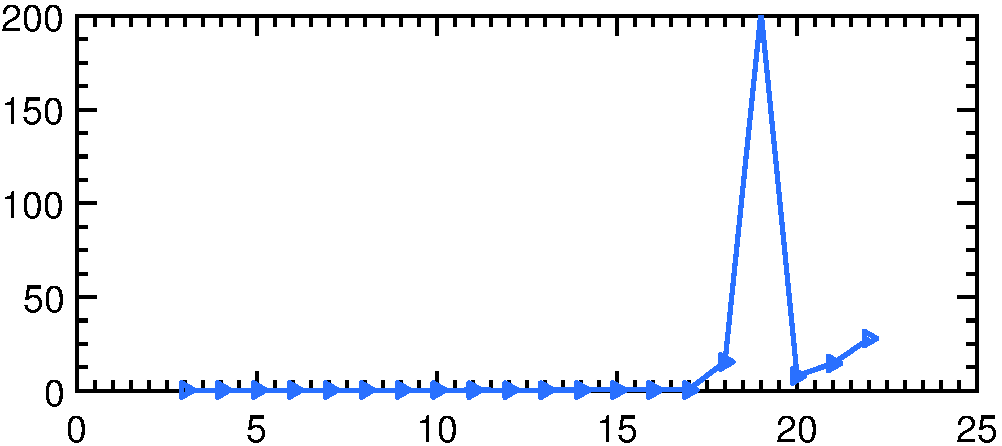
\includegraphics[width=.5\columnwidth]{benchmark}
	\caption[Running time]{X-axis: number of landmarks, Y-axis: elapsed time in seconds. Running time starts to grow explosively at $n=17$ and becomes $200s$  at  $n=19$  suddenly}
	\label{fig:elaspe}.
\end{figure}
		

\begin{appendices}
\section{Lab Code}
My codes are somewhat lengthy, so I just put some important code, hope not to impact the compactness of this report.
	\subsection{Crawling Data of CHINA Landmarks}
	\lstinputlisting[language=Python]{./code/test.py}
	\subsection{Solve By Sage}
	\lstinputlisting[language=Python]{./code/sage.py}
	\subsection{Draw on GMap}
	\lstinputlisting[language=Matlab]{./code/lOptHw.m}	
	%\textbf{\textcolor[rgb]{0.98,0.00,0.00}{Input matlab source:}}
	
	%some more text \textcolor[rgb]{0.98,0.00,0.00}{\textbf{Input C++ source:}}
	%\lstinputlisting[language=C++]{./code/mcmthesis-sudoku.cpp}
	
%			\section{Landmarks Around HangZhou }
%			\begin{longtable}{|l||l|l|} \hline
city & latitude & longitude \\ \hline \hline
$\text{\texttt{Hangzhou}}$ & $30.274085$ & $120.15507$ \\ \hline
$\text{\texttt{Ningbo}}$ & $29.868336$ & $121.54399$ \\ \hline
$\text{\texttt{Wenzhou}}$ & $27.993828$ & $120.699362$ \\ \hline
$\text{\texttt{Jiaxing}}$ & $30.753924$ & $120.758543$ \\ \hline
$\text{\texttt{Huzhou}}$ & $30.894348$ & $120.086823$ \\ \hline
$\text{\texttt{Shaoxing}}$ & $29.995762$ & $120.586109$ \\ \hline
$\text{\texttt{Jinhua}}$ & $29.079175$ & $119.647421$ \\ \hline
$\text{\texttt{Quzhou}}$ & $28.97008$ & $118.859457$ \\ \hline
$\text{\texttt{Zhoushan}}$ & $29.985295$ & $122.207216$ \\ \hline
$\text{\texttt{Taizhou}}$ & $28.65638$ & $121.42076$ \\ \hline
$\text{\texttt{Xiaoshan}}$ & $30.168016$ & $120.414929$ \\ \hline
$\text{\texttt{Jiande}}$ & $29.474871$ & $119.281164$ \\ \hline
$\text{\texttt{Fuyang}}$ & $30.048692$ & $119.960076$ \\ \hline
$\text{\texttt{Yongning{ }Rd}}$ & $30.4682595$ & $120.308662$ \\ \hline
$\text{\texttt{Lin'an}}$ & $30.233873$ & $119.724733$ \\ \hline
$\text{\texttt{Yuyao}}$ & $30.037192$ & $121.154634$ \\ \hline
$\text{\texttt{Cixi}}$ & $30.169665$ & $121.266579$ \\ \hline
$\text{\texttt{Fenghua}}$ & $29.655143$ & $121.406995$ \\ \hline
$\text{\texttt{Rui'an}}$ & $27.778657$ & $120.655148$ \\ \hline
$\text{\texttt{Deqing}}$ & $30.623883$ & $120.289015$ \\ \hline
$\text{\texttt{Haining}}$ & $30.510659$ & $120.680757$ \\ \hline
$\text{\texttt{Pinghu}}$ & $30.677233$ & $121.015142$ \\ \hline
$\text{\texttt{Tongxiang}}$ & $30.630173$ & $120.565099$ \\ \hline
$\text{\texttt{Zhuji}}$ & $29.708692$ & $120.246863$ \\ \hline
$\text{\texttt{Shangyu}}$ & $30.033121$ & $120.868122$ \\ \hline
$\text{\texttt{Shengzhou}}$ & $29.56141$ & $120.831026$ \\ \hline
$\text{\texttt{Lanxi}}$ & $29.208919$ & $119.460526$ \\ \hline
$\text{\texttt{Yiwu}}$ & $29.306757$ & $120.07514$ \\ \hline
$\text{\texttt{Dongyang}}$ & $29.289648$ & $120.241566$ \\ \hline
$\text{\texttt{Yongkang}}$ & $28.888555$ & $120.047651$ \\ \hline
$\text{\texttt{Jiangshan}}$ & $28.737223$ & $118.626974$ \\ \hline
$\text{\texttt{Wenling}}$ & $28.372506$ & $121.385604$ \\ \hline
$\text{\texttt{Linhai}}$ & $28.858457$ & $121.145046$ \\ \hline
$\text{\texttt{Lishui}}$ & $28.46763$ & $119.922796$ \\ \hline
$\text{\texttt{Longquan}}$ & $28.07465$ & $119.141474$ \\ \hline
$\text{\texttt{Shanghai}}$ & $31.230416$ & $121.473701$ \\ \hline
$\text{\texttt{Nanjing}}$ & $32.060255$ & $118.796877$ \\ \hline
$\text{\texttt{Wuxi}}$ & $31.49117$ & $120.31191$ \\ \hline
$\text{\texttt{Xuzhou}}$ & $34.205768$ & $117.284124$ \\ \hline
$\text{\texttt{Changzhou}}$ & $31.811226$ & $119.974062$ \\ \hline
$\text{\texttt{Suzhou}}$ & $31.298979$ & $120.58529$ \\ \hline
$\text{\texttt{Nantong}}$ & $31.980172$ & $120.894291$ \\ \hline
$\text{\texttt{Lianyungang}}$ & $34.596653$ & $119.221611$ \\ \hline
$\text{\texttt{9{ }Xueyuan{ }Rd}}$ & $33.598607$ & $119.0033924$ \\ \hline
$\text{\texttt{Yancheng}}$ & $33.347316$ & $120.16366$ \\ \hline
$\text{\texttt{Yangzhou}}$ & $32.394213$ & $119.412947$ \\ \hline
$\text{\texttt{Zhenjiang}}$ & $32.187849$ & $119.425836$ \\ \hline
$\text{\texttt{Taizhou}}$ & $32.455536$ & $119.922933$ \\ \hline
$\text{\texttt{745{ }Country{ }Rd}}$ & $34.3147372$ & $118.901079$ \\ \hline
\end{longtable}		
\end{appendices}

	
\end{document}